% Drawing 154/05-10 -- folder 154, batch 05, archive page 83 (PDF page 84).
% Transcription: en haut à gauche, un disque au crayon traversé de six droites en noir et d'une courbe orange, qui les coupe presque toutes en deux paquets près de deux points
% Kind: disk with six lines and an orange curve. Method 2 (schematic redraw from the facsimile). Status: partial.
% Notes: Pencil circle (its lower arc gone over more heavily); the orange curve sags across the disk from left to right; six black strokes: two straight ones crossing the upper left of the disk and meeting the orange curve near its left end, three bending down to the right and meeting it near a second point, where they bunch, one running along the underside of the orange curve. The two bunching points are drawn as common points (as the transcription describes them); on the page the strokes pass within a stroke's width of each other there. Ends inside the disk are drawn where the strokes stop. Redrawn 2026-11-12 (issue 128): to check again.
% Coordinates: 1 unit = 1 mm = 1/100 of the crop width (bbox in page fractions: [0.76, 0.41, 0.9, 0.51]).
% Redrawn by Claude (claude-fable-5-2), issue #128, 2026-11-12; not checked by a human; not compiled (no TeX in the session).
% Rights: reproduces part of the work -- behind RENDER_TRANSCRIPTS, never published by itself.
\documentclass[tikz,border=3pt]{standalone}
\usepackage{amsmath,amssymb}
\usetikzlibrary{patterns,arrows.meta}
\tikzset{Or/.style={orange!90!black}, pencil/.style={black!45}, struck/.style={black!35}, mpt/.style={circle,draw,inner sep=1.3pt}, pt/.style={circle,fill,inner sep=0.9pt}, opt/.style={circle,draw,fill=white,inner sep=1.1pt}}
\begin{document}
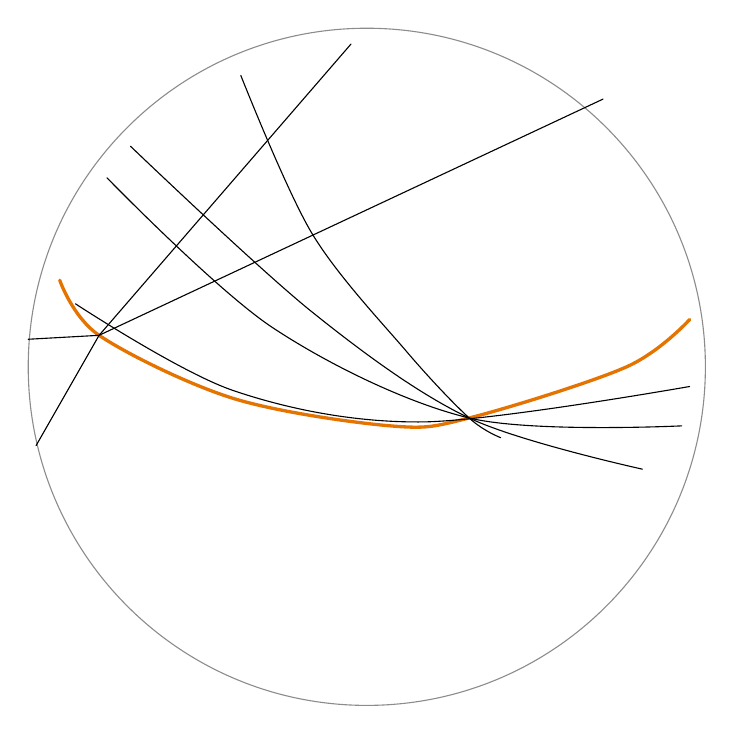
\begin{tikzpicture}[x=1mm,y=1mm,line cap=round,line join=round,font=\scriptsize]
\draw[pencil] (47,-47) circle[radius=43];
\draw[Or,very thick] plot[smooth, tension=0.55] coordinates {(8,-36) (13,-43) (30,-51) (50,-54.5) (60,-53.5) (80,-47) (88,-41)};
\draw (45,-6) -- (13,-43) -- (5,-57);
\draw (77,-13) -- (13,-43) -- (4,-43.5);
\draw plot[smooth, tension=0.55] coordinates {(31,-10) (40,-30) (52,-45) (60,-53.5) (64,-56)};
\draw plot[smooth, tension=0.55] coordinates {(17,-19) (40,-40) (60,-53.5) (82,-60)};
\draw plot[smooth, tension=0.55] coordinates {(14,-23) (35,-42) (60,-53.5) (87,-54.5)};
\draw plot[smooth, tension=0.55] coordinates {(10,-39) (30,-50) (54,-54) (88,-49.5)};
\end{tikzpicture}
\end{document}
